
Algebra today is taught chronologically by example. 
First groups, then rings, then fields, then modules,
then bigger groups, then crazier rings, then fusing groups and rings with
outside influences like topology, analysis, and geometry.  Today there are
few general-practice algebraist.  There are instead geometric group theorist,
algebraic geometers, commutative ring theorist, representation theorist, non-associative algebraist,
computational algebraist (that's me), and even those topics are too general for any one
theorist to master. 

It bucks tradition (set out by Noether) to change this approach to algebra.
Chances are high that the books that brought you here already laid out the subject
in this order.
But I speculate that there is a place in the sciences for a view of algebra 
as a whole.  What is it that algebra does? Like many who work in math 
a likely response has a does of calculated propaganda to impress your 
parents, funding agency, or quite the passenger next to you. This text 
offers some clues about making that response a bit more honest in intention.
I divide all of algebra into a 3 phase flow chart.
\begin{center}
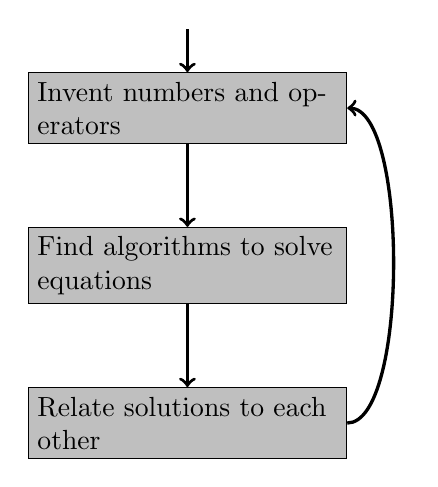
\begin{tikzpicture}
    \node[text width=1.5in, draw,fill=black!25] (a) at (0,0) {Invent numbers and operators};
    \node[text width=1.5in, draw,fill=black!25] (b) at (0,-2) {Find algorithms to solve equations};
    \node[text width=1.5in, draw,fill=black!25] (c) at (0,-4) {Relate solutions to each other};
    \draw[very thick,->] (0,1) -- (a);
    \draw[very thick,->] (a) -- (b);
    \draw[very thick,->] (b) -- (c);
    \draw[very thick,->] (c) edge[looseness=0.5,out=0,in=0] (a);
\end{tikzpicture}
\end{center}
